% !TEX root = ../thesis.tex


\chapter{Beam Propagation using the Hankel Transform}
% \label{cha:beam_propagation}

In this chapter I will briefly show how the trapping geometry presented before could be realised in an experiment.
The two ring beams can be produced with axicon lenses. I have programmed a simple beam propagation for cylindrical beams. This tool can be found on my personal GitHub page\footnote{\url{github.com/AvonHaaren}} and was programmed in \Cpp and Python.

\section{Theory -- Fourier Optics}
Fourier optics in a mathematical approach to the propagation of light through free space and variuos media. In Fourier optics, the light field is decomposed into a sum of plane waves, each of which can be propagated through an arbitrary linear optical system independently. Afterwards, the components are superimposed to give the light field after the system. In two dimensions, this is done by using the Fourier transform
\begin{align}
    \mathcal{F}\left\{f(x,y)\right\} = F(\nu_x,\nu_y) &= \iint \diff{x} \diff{y}\; f(x,y) \exp\!\left(2\pi i (x\nu_x + y\nu_y)\right) \\
    f(x,y) &= \iint \diff{\nu_x} \diff{\nu_y}\; F(\nu_x,\nu_y) \exp\!\left(-2\pi i (x\nu_x + y\nu_y)\right)
\end{align}
In the case of free space propagation, the transfer function $H(\nu_x,\nu_y,\Delta z)$ is fully expressed by the spatial frequencies $\nu_x$ and $\nu_y$. Using this, we can express the electric field after a distance $\Delta z$ through
\begin{align}
    E(x,y,\Delta z) = \iint \diff{\nu_x} \diff{\nu_y}\; H(\nu_x,\nu_y,\Delta z) \mathcal{F}\left\{E(x,y,0)\right\} \exp\!\left(-2\pi i (x\nu_x + y\nu_y)\right)
\end{align}

\subsection{Cylindrical Symmetry}
If the light field and optical system are cylindrically symmetric, the Fourier transform in the equation above can be replaced by the Hankel transform of zero order:
\begin{align}
    G(\rho) &= 2\pi\int_0^\infty \diff{r}\; g(r) r J_0(2\pi r \rho) \\
    g(r) &= 2\pi \int_0^\infty \diff{\rho}\; G(\rho) \rho J_0(2\pi r \rho)
\end{align}
Here, $g(r)$ is the field in real space, $G(\rho)$ the transformed field in reciprocal space and $J_0$ is the Bessel function of zero order. $\rho$ is the spatial frequency in radial direction, where $2\pi\rho = \kappa$ is the radial wavenumber. For numerical calculations, this reduction to a one-dimensional problem is highly beneficial.

\subsection{Transfer Functions of Optical Elements}
\paragraph{Spherical Lens} ~\\
The transfer function of a spherical lens is given by
\begin{equation*}
    H_\text{TL}(r) = \exp\!\left(-i\pi\frac{r^2}{f\lambda}\right)
\end{equation*}
where $f$ is the focal length and $\lambda$ the wavelength of the light.

\paragraph{Axicon} ~\\
An axicon has a transfer function
\begin{equation*}
    H_\text{A}(r) = \exp\!\left(-\frac{2\pi r}{\lambda}(n - 1)\tan(\alpha)\right)
\end{equation*}
where $n$ is the refractive index of the axicon and $\alpha$ is the opening angle, as shown in \cref{fig:axicon}. A constant phase factor depending on the thickness of the axicon has been omitted.
\begin{figure}[htbp]
    \centering
    \usetikzlibrary{positioning,calc}
\tikzset{beam/.style={color=red!70!black}}
\begin{tikzpicture}[scale=2.5]
    \coordinate (T) at (0,0.5);
    \coordinate (B) at (0,-0.5);
    \coordinate (Tip) at (0.185,0);
    \draw (T) -- (B) -- (Tip) -- cycle;
    \draw[-latex,dashdotted] (-0.5,0) -- (4.5,0) node[right] {$z$};
    \draw[-latex] (0,-0.5) -- (0,0.6) node [above] {$r$};
    \draw (0,-0.8) arc (-90:-110:0.3);
    \draw[densely dotted] (B) -- ($(Tip)!1.57!(B)$);
    \draw[densely dotted] (B) -- (0,-0.8) node [midway,right] {$\alpha$};
    \foreach \y in {0.01,0.02,0.0325,0.045,0.065,0.085,0.115,0.145}
    \foreach \M in {1,-1}
    {
        \coordinate (IS) at (intersection cs: first line={(-0.5,\y*\M) -- (2,\y*\M)},second line={(0,\M) -- (Tip)});
        \coordinate (IS1) at ($(IS) + (4,-\M*4*0.176)$);
        \coordinate (IS2) at (intersection cs: first line={(IS) -- (IS1)}, second line={(4,-1) -- (4,1)});
        \draw[beam] (-0.5,\y*\M) -- (IS) -- (IS2);
    }
\end{tikzpicture}
    \caption{Axicon Lens}
    \label{fig:axicon}
\end{figure}

\paragraph{Free Space} ~\\
The free space transmission function depends only on the coordinates in reciprocal space:
\begin{equation}
    H_\text{FS}(\rho, \Delta z) = \exp\!\left(\frac{2\pi i \Delta z}{\lambda}\sqrt{1 - (\lambda \rho)^2}\right)
\end{equation}
Notably, for $\rho^{-1} > \lambda$, transmission is exponentially suppressed. This expresses the fact that structures smaller than a wavelength are not resolvable.


\subsection{Numerical Evaluation}
To calculate the Hankel transform and its inverse, we discretise real and reciprocal space up to maximum values $r_\text{max}$ and $\rho_\text{max}$ in regular intervals with spacings $\delta r$ and $\delta \rho$ given by
\[
    \delta r = \frac{r_\text{max}}{N}, \quad \delta \rho = \frac{\rho_\text{max}}{N}
\]
where $N$ is the grid size.
Then we have
\begin{align}
    G(\rho) &= 2\pi \delta r \sum_{i = 0}^N r_i  g(r_i) J_0(2\pi r_i \rho) \\
    g(r) &= 2\pi \delta \rho \sum_{i = 0}^N \rho_i  G(\rho_i) J_0(2\pi r \rho_i)
\end{align}
To save computation time, the Bessel function can be pre-evaluated on a $N\times N$ grid. However, at high resolutions, the memory consumption of this becomes too large, also resulting in higher cache miss rates. We therefore only evaluate the Bessel function on a grid of size $M$ with maximum $2\pi r_\text{max} \rho_\text{max}$. Interpolation between these values is much faster than calculating the exact value of $J_0(x)$ in the transformation.


\section{Tested Setup and Results}
To test an optical system with an arbitrary number of elements, the initial electric field is propagated to the $n$-th optical element using the Hankel transform and the free space propagator. At the location of the optical element, the field is transformed back into real space, the transfer function of the element is applied and then the field can be propagated to the next element etc.

We adapt the setup from Hueck et al. \cite{PhysRevLett.120.060402}, using one axicon \cite{McLeod} to split the initial gaussian into a ring, another axicon in combination with a long focal length spherical lens to invert it and then a third, movable axicon to produce a collimated ring that can have a varying radius. This is shown in \cref{fig:axicon_setup}. In the setup that we want to use and that is simulated, there is an additional $5\times$ demagnification stage after the third axicon.
\begin{figure}[htbp]
    \centering
    \begin{tikzpicture}
    \node[anchor = south west, inner sep=0] (Image) at (0,0) {\includegraphics[page=2,trim=160 590 55 70,clip]{Evap/AxiconSetup/File}};
    \begin{scope} [x={(Image.south east)},y={(Image.north west)}]
        \node[rectangle, rounded corners,draw=none,inner sep=1pt] at (0.225,0.152) {$f=\SI{400}{mm}$};
        \node[rectangle, rounded corners,draw=none,inner sep=1pt] at (0.922,0.152) {\parbox{1.5cm}{\centering Image Plane}};
        \node[rectangle, rounded corners,draw=none,inner sep=1pt] at (0.074,0.89) {$\SI{10}{\degree}$ Axicon};
        \node[rectangle, rounded corners,draw=none,inner sep=1pt] at (0.27,0.89) {$\SI{10}{\degree}$ Axicon};
        \node[rectangle, rounded corners,draw=none,inner sep=1pt] at (0.8,0.89) {Movable $\SI{2}{\degree}$ Axicon};
    \end{scope}
\end{tikzpicture}
    \caption[Optical setup to create a ring beam with dynamically adjustable radius]{Adapted from \cite{axiconSM}. Optical setup to create a ring beam with dynamically adjustable radius. Not shown here is an additional microscope that demagnifies the beam from the image plane to the target plane.}
    \label{fig:axicon_setup}
\end{figure}
The position of the first axicon is defined as $z=0$. The \SI{400}{mm} lens is positioned at $z=\SI{85}{mm}$ with the second axicon behind it at $z=\SI{95}{mm}$. The third axicon can be moved between $z=\SI{585}{mm}$ and $z=\SI{625}{mm}$ \todo{check if correct}.
The initial gaussian beam has a wavelength of \SI{770}{nm} the position of its waist relative to $z=0$ as well as the waist size can be varied.

\begin{figure}[htbp]
    \centering
    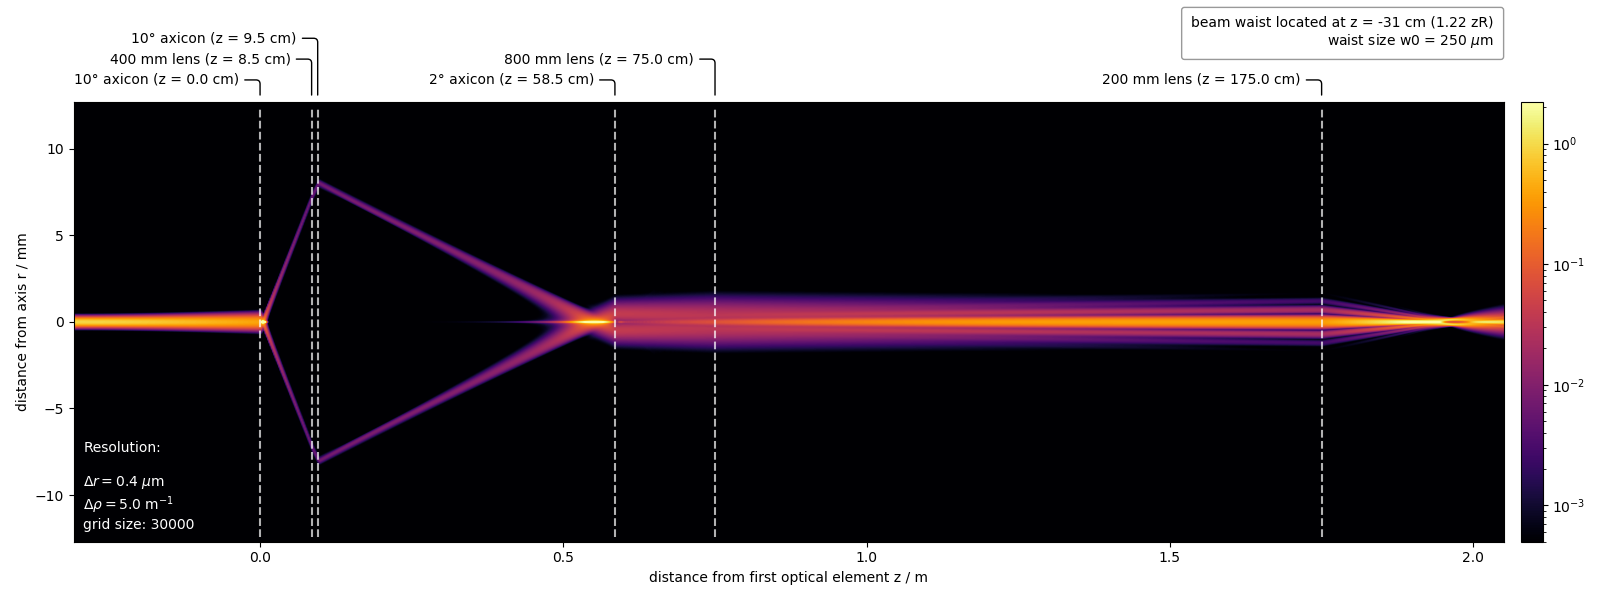
\includegraphics[width=\textwidth]{Evap/AxiconBeam/plot}
    \caption{Example of a beam resulting from the setup above. \textbf{PRELIMINARY, WILL BE SWAPPED OUT FOR THE FINAL VERSION}}
    % \label{fig:axiconBeam}
\end{figure}

\begin{figure}[htbp]
    \centering
    \begin{subfigure}[t]{0.49\textwidth}
        \centering
        \missingfigure[figwidth=.9\linewidth]{Closeup of the focus region}
        \caption{Close-up image of the beam in the focus region}
    \end{subfigure}
    \begin{subfigure}[t]{0.49\textwidth}
        \centering
        \missingfigure[figwidth=.9\linewidth]{Intensity Plot at the focus, with fitted power law}
        \caption{Resulting ring intensity at the focus position. A power-law curve has been fitted to the data. \textbf{VALUE MISSING}}
    \end{subfigure}
    \caption{Ring beam at the focus position with a resulting diameter of \textbf{VALUE MISSING}.}
    % \label{fig:axiconBeamResult1}
\end{figure}
